%===================================== CHAP 2 =================================

\chapter{Prestudies}

\section{Customer input}

In the first meeting with the customer, the group received input about the overall structure of the product, as well as the research required. The customer put emphasis on a few factors of importance when designing the application. The protocol implementation had to be modularized in such a way that additional protocol support could be added with ease at a later time. A graphical administration interface was also required, to be able to review broker data and adjust publisher/subscriber mappings. Additionally, extensive research had to be done, both to learn how the different protocols work, and to get an overview of the publish-subscribe pattern in general. These factors had an impact when choosing what sort of solution the group would develop. It also affected the development and research methodology.

The application was meant to be used internally in the Norwegian Armed Forces. Due to this, the group didn't have to consider the targeted user group in any way. The customer would field test the application at a later time. Thus, the only focus in that area was the feedback acquired from the customer.

\section{Publish-subscribe}

The implementation of the product had to be structured in a publish subscribe messaging pattern. In this pattern, the publishers does not send messages to specific receivers. Instead, messages are placed into categories, and sent to all receivers who subscribes to the category. Publishers and subscribers are separated, as subscribers do not know which publishers, if any, exists. In the same manner, publishers have no insight into which, if any subscribers exists to the category.

There are two main types of patterns used by the different protocols. The most popular one is using topics or queues. This method allows a subscriber to subscribe to a certain topic. Whenever someone posts a message in that topic, all subscribers on that topic receive the same message. Using queues, the idea is extended by setting up a hierarchy. The function of the topic hierarchy is to allow publishing and subscribing to different levels of the hierarchy. Basically, when subscribing to a topic, one will also receive messages sent to all subtopics. The other type of message subscription is using content filtering. Using this method, a subscriber will only receive a message if its contents match some given filtering criteria requested by the subscriber.

The general publish-subscribe pattern is visualized in this figure.

\begin{center}
  \begin{figure}[ht]
    \makebox[\textwidth]{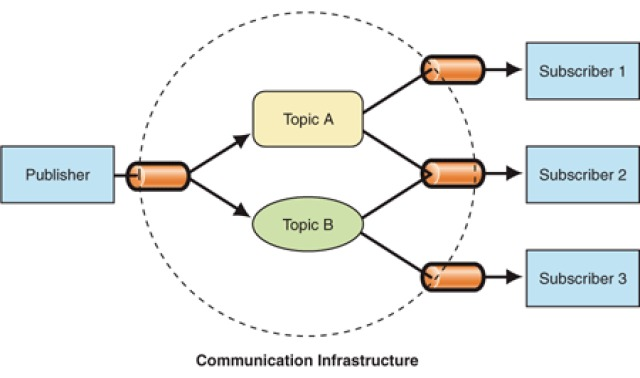
\includegraphics[width=\textwidth]{fig/publish-subscribe.jpg}}
    \caption{Publish-subscribe}
    \label{fig:publish-subscribe}
  \end{figure}
\end{center}

\section{Protocols}

The following sections describe the protocols the system were to support, in descending order of importance.

\subsection{WSNotification}

WSNotification\footnote{\url{https://www.oasis-open.org/committees/wsn/}} is a messaging protocol developed by OASIS.\footnote{\url{https://www.oasis-open.org/}} It is a protocol that implements the publish-subscribe pattern over HTTP. The protocol uses SOAP to send XML messages over the network. The complete standard can be found here. \footnote{\url{http://docs.oasis-open.org/wsn/wsn-ws_base_notification-1.3-spec-os.htm}}

\subsection{AMQP}
Advanced Message Queuing Protocol (AMQP)\footnote{\url{http://www.amqp.org/}} is a binary protocol for sending messages over a computer network. The protocol is built for handling the queuing of messages and routing (including publish-subscribe handling) in a reliable and secure way. The main funding and development of AMQP comes from the financial sector.

\subsection{MQTT}
MQTT\footnote{\url{http://mqtt.org/}} is a publish-subscribe based protocol. It has the advantage of being lightweight and uses a minimal footprint wherever it can. The protocol also minimizes its use of bandwidth. MQTT has gained a lot of popularity the last years due to its exceptional properties which makes it suitable for everything from embedded system to big implementations like the Facebook Messenger\footnote{\url{https://www.facebook.com/notes/facebook-engineering/building-facebook-messenger/10150259350998920}}. This protocol was removed from the requirements in the mid stages of the project, due to time issues.

\section{Existing solutions}

Following is the evaluation of current existing solutions, that more or less covers the product description. The customer had little to no experience with any of the existing solutions, other than knowledge of their existence, and tasked us to make an evaluation of the applications in question.

\subsection{Apache Apollo}

Apache Apollo\footnote{\url{http://activemq.apache.org/apollo/}} is an open source project maintained by the Apache\footnote{\url{http://www.apache.org}} foundation and commercially supported by Red Hat \footnote{\url{http://www.redhat.com/}}. This application distinguishes itself from the existing solutions presented below, in the way that it is a complete, protocol agnostic broker, that translates freely between AMQP, MQTT, OpenWire and STOMP. It is an up to date project, that is continually updated by the developer team.

Apache Apollo can be considered as the next generation of the older Apache ActiveMQ broker\footnote{\url{http://activemq.apache.org}}. It is a complete reimplementation of the old broker built on more modern programming concepts and a more efficient message handler.    

\subsubsection{Evaluation}

Initially, the group set up an instance of Apache Apollo and read through both the user and developer documentation. It became clear that Apollo was a very well written broker, and covered many of the requirements given by the customer.

The internals of the message queuing and message translation systems were very well designed. It uses a non-blocking reactor thread model, which keeps all threads running and consumes tasks asynchronously, allowing for a fast message processing rate. Another important factor was that Apollo dynamically converts large message queues from actual objects to pointer references, when the queue becomes large. This helps mitigate the memory limits of the Java Virtual Machine, and allows Apollo to maintain queues larger than what a regular in-memory queue system would have. There was one issue with Apollo however. A lot of the functionality is written in Scala\footnote{\url{http://www.scala-lang.org/}}. None of the group members had any prior experience with the programming language.

\subsection{RabbitMQ}

RabbitMQ\footnote{\url{https://www.rabbitmq.com}} is an open source project created and maintained by Pivotal Software\footnote{\url{http://www.pivotal.io}}, which provides commercial support for the product. The software is mainly written for version 0.9 of AMQP, but supports version 1.0 via an experimental plug-in. There is also plug-in support for MQTT. RabbitMQ provides a large amount of bindings for a wide range of different programming languages. RabbitMQ and its plugins are written in the Erlang programming language.

\subsubsection{Evaluation}

RabbitMQ and its plugins are implemented in a programming language and a programming paradigm that was not preferred by the customer. Thus, it would not be practical to build upon this solution. Additionally, no-one in the group had previous experience with Erlang. Therefore, the group ended up concluding that further research was unnecessary.

\subsection{WS-Nu}

WS-Nu is a project developed as an assignment at NTNU. It is an implementation of the WSN protocol written in Java. It fully incorporates support for a large part of the WSN standard.

\subsubsection{Evaluation}

WS-Nu is a well written piece of software, which accomplishes many of the tasks of this project. Additionally, it was recommended for research and use by the customer.

\subsection{MicroWSN and NFFIPlayer}

MicroWSN and NFFIplayer are both software developed and provided by FFI. MicroWSN is an implementation of a WSN broker. NFFIPlayer is a graphical interface for testing MicroWSN. The package was created by FFI for testing in the field. However, the implementation is incomplete, and lacks several features that a complete implementation should have.

\subsubsection{Evaluation}

The package was not considered for further development, due to its incompleteness, and that it is purely a broker for WSN. However, due to the graphical interface provided, it proved useful for the group while testing the WSNotification implementation.

\section{Overall evaluation}

The main outcome of the prestudy, was the discovery of Apollo. It proved to be a solution it was possible to expand further, and the option of choosing that appeared. Depending on whether we would develop our own, custom tailored broker, or expand on the Apollo project would determine what sort of architecture draft we would develop. One issue with Apollo however, proved to be the massive code base and previous work done on the implementation. It was clear that the quality of the code, as well as the amount of work put into the product, would be a challenge. A lot of the code base were hard to understand, due to the massive amount of references to other parts of the software. Additionally, the web interface was built using Scala, a language none of the group members had any experience with.

The group chose to introduce an extended research phase, in order to make a final decision regarding Apollo. This was based on an initial risk analysis of what would become a research project. These risks would lay the foundation of the research process, and define the different areas to study further. The risk analysis is shown below, and a more detailed description of the methodology is explained in chapter 3.

\begin{table}[h]
\centering
\resizebox{\textwidth}{!}{%
\begin{tabular}{|p{0.3\linewidth}
                |p{0.2\linewidth}
                |p{0.2\linewidth}
                |p{0.3\linewidth}|}
\hline
Description                                 & Likelihood (1-9) & Impact (1-9) & Importance (Likelihood * Impact) \\ \hline
Apollo being too complex                    & 5                & 9            & 45                               \\ \hline
Unable to learn Scala                       & 2                & 6            & 12                               \\ \hline
Unable to implement additional modules      & 5                & 9            & 45                               \\ \hline
Too much time required to implement Apollo  & 4                & 5            & 20                               \\ \hline
\end{tabular}
}
\caption{Risk analysis for Apollo}
\label{fig:risk_analysis_apollo}
\end{table}

\section{Planned solution}

In order to design a final solution, all the factors evaluated so far would had to be considered. After the extended research phase, the final decision was to discard Apollo completely. This was due to that the issues mentioned earlier, proved to be larger than initially expected. The risk of not being able to complete the Apollo implementation was simply too large. The result of the research work done on Apollo, is more thoroughly covered in appendix A.

Plan B was to develop a completely new protocol brokering solution. However, the group also chose to use WS-Nu as the WSN implementation of the product. 

The two major development tasks, was to create a web interface and the brokering solution in itself. The initial architecture sketch was strongly influenced by Apollo, due to its robustness and the sheer quality of the product. A simplified version of it were created, and the sketch is composed of the following building blocks.

\begin{center}
  \begin{figure}[ht!]
    \makebox[\textwidth]{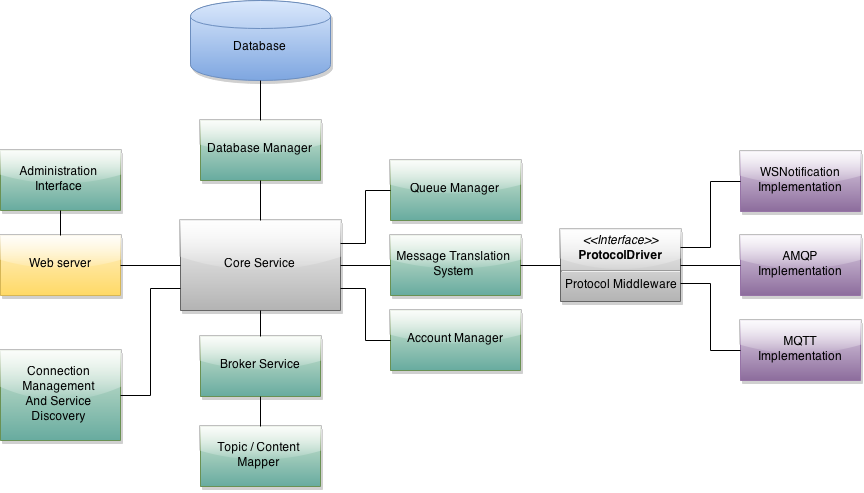
\includegraphics[width=\textwidth]{fig/arch_proposal_aleks.png}}
    \caption{Pub-Sub Broker Sketch}
    \label{fig:arch_proposal}
  \end{figure}
\end{center}

\section{Tools}

Following is the list of all the tools used in this project. This includes tools used for communication, document sharing and development.

\subsection{Skype}

Skype\footnote{\url{www.skype.com}} was the main tool used for communication with the customer. Meetings were held using the group call feature of Skype. Communication within the group was done using both group calls, as well as the instant messaging feature within Skype. The tool was convenient to use both for the customer and the group. It provided all the communication features needed, both voice communication and a textual chat.

\subsection{Java}

The customer prefered that the main part of development was done using Java. Java is a programming language widely used in software development. The group chose version 8 as the target, which is the newest version. One of the main benefits of choosing Java and the Java Virtual Machine (denoted as JVM) as the language and platform is the the broker could run on every system where the JVM is available. This means that the broker will not be affected by different hardware architectures or operating systems as long as they are supported.

\subsection{Spring MVC}

Spring MVC\footnote{\url{www.spring.io}} is a model view controller framework developed in Java. Its a modern framework mostly used for development of web-based applications. The framework was chosen after a quick evaluation of different possibilities. It was chosen because it was easy to learn, and gave us exactly what was required, with a small amount of work to set up.

\subsection{JavaDoc}

In this project, the group has chosen to use JavaDoc, an automatic, comment based documentation tool to provide developer documentation of the code base. JavaDoc is supported in most Java Integrated Development Environments (IDE), and allows for easy generation and updating of developer documentation. JavaDoc is the standard documentation tool for development in Java. Thus, few good alternatives exist that covers the same functionality, and the tool was an obvious choice in this project.

\subsection{IntelliJ IDEA}

IntelliJ IDEA\footnote{\url{www.jetbrains.com/idea/}} is a Java integrated development environment(IDE). It contains a wide array of useful built-in functions for development in Java. It also includes support for build systems like Maven and Gradle. Version control systems are also well integrated in the tool.

There exists many different development environments. Everything from simple text editors, to fully integrated development environments might be used. Considering development in Java however, one achieves some advantages by using a big platform. Both code completion, and functions for compiling code in the environment, makes the development process easier and faster. The group considered mainly three alternatives when considering the environment. IntelliJ, Eclipse\footnote{\url{www.eclipse.org}} and Netbeans\footnote{\url{www.netbeans.org}}. The choice came down to mainly two deciding factors. Both eclipse and Netbeans suffer from having a confusing amount of plugins for different tasks, where as the built in features of IntelliJ are widely cohesive. Secondly, IntelliJ was the first to release support for Java 8 and has proven to be stable and efficient over time.

\subsection{Apache Maven}

Apache Maven\footnote{\url{http://maven.apache.org/}} is a software solution for handling structuring, building and testing of Java projects. Maven also provides the developers with a package manager which can be used for fetching both own or third party libraries and adding them automatically into the system. It is well implemented and widely used. Most Java Development Environments like Eclipse and IntelliJ supports Maven integration.

\subsection{TestNG}

TestNG\footnote{\url{www.testng.org}} is a framework used for writing unit tests in Java. Compared to the more commonly used JUnit, TestNG is implemented with better handling of tests that requires threads, easier parametrized tests and the ability to more efficiently use data providers in the tests. TestNG also integrates out of the box with both Maven and Intellj IDEA.

\subsection{Git}

Version control is important when working on a project like this. The group chose to use Git\footnote{\url{http://en.wikipedia.org/wiki/Git_(software)}}, in collaboration with GitHub\footnote{\url{www.github.com)}}, a cloud hosted, distributed revision control system that allows all team members to access the code. Git provides complete history and version control, with complete offline support, as the Git working directory acts as a complete repository.

% Someone please read if engrish makes sense.
There are other distributed version control systems (DVCS) available. However, every group member had experience with both Git and GitHub prior to the start of the project and the entire group agreed that using these services would be the best choice. Another important part of the decision was that the group meant that it would be counterproductive to research and learn a different version control system, as the time should rather be spent on researching and working on the product.

% Someone please read if engrish makes sense.
\subsection{Jenkins}
Jenkins\footnote{\url{http://jenkins-ci.org/}} is an open source continuous integration tool. Continuous integration is a helping concept for software development which can be used for automatic testing and reporting, automatically do maintenance and other routine work and deploy software automatically. 

For the groups project Jenkins was used as a automatic test runner with full reporting from a build and automatic deployment of the latest stable release of the system on our test server. A automatic test run or deployment was triggered by integrating Jenkins with GitHub.

Jenkins does also provide out of the box integration with Maven, Git and TestNG.

\subsection{Gantt project}

Gantt project\footnote{\url{http://www.ganttproject.biz/}} is a tool used to create gantt charts. It is a simple chart creation tool exclusively made for creating clean and structured gantt diagrams. The group had prior experience with tool, and the tool was chosen based on that.

\subsection{Google Drive}

Google Drive\footnote{\url{https://drive.google.com/}} is a platform for sharing documents. Drive supports all necessary types of files, as well as supporting real time cooperation on documents. The simplicity of Google Drive is what makes it an attractive platform. The ability to simply upload a file to the website, and instantly having it shared with everyone in the group, is both efficient and easy to grasp. Compared to using email for file sharing, or storage on a physical medium, a cloud solution is more suitable. 

In the case of this project, Drive was used to share all text and image files used in the report. It also served as the main platform for sharing and collaborating on time-tables and agendas for meetings, both with the customer and supervisor. There were no other alternatives that covered all the functionality of Drive.

\subsection{LaTeX\ and ShareLatex}

ShareLatex\footnote{\url{http://sharelatex.com}} is an online platform for collaborative editing of LaTeX documents. Furthermore, LaTeX is a typesetting system, designed for production of technical and scientific documentation.

The group chose to use LaTeX as the way of constructing the report. Compared to other solutions like Microsoft Word, it allows you to generate clean and well formed documents. It also opens the opportunity for automatically generating a front page and table of contents. In the end however, the choice fell on LaTeX due to it being better, and more professional looking than many of it's alternatives.

ShareLatex can in some ways be compared to Google Drive. The difference however, is that it is exclusively built for sharing LaTeX documents. It features the ability to cooperate on the documents in real time, as well as compile and preview documents.

\section{Risk analysis}

The groups risk assessment was made early in the planning phase. The table (fig. \ref{fig:risk_analysis}) shows what was considered to be the most likely events happening, as well as preventive actions. Upon inspection of each of the risks, a number between 1 and 10 was chosen for the likelihood of the case happening, as well as the potential impact it would have. The final rank of the risk was defined as these two numbers multiplied. When a risk was identified we included a remedial action, to reduce the impact.

\begin{longtable}{@{\extracolsep{\fill}}|p{0.2\linewidth}
                |p{0.15\linewidth}
                |p{0.1\linewidth}
                |p{0.15\linewidth}
                |p{0.225\linewidth}
                |p{0.225\linewidth}|@{}}
\hline
\textbf{Description}                                 & \textbf{Likelihood (1-9)} & \textbf{Impact (1-9)} & \textbf{Importance (Likelihood * Impact)} & \textbf{Preventice Action}    & \textbf{Remedial Action} \\ \hline

Delivering an unsatisfying product.  & 3 & 9 & 27 & Frequent customer meetings. Make sure to have a mutual understanding of the goal of the progress. &   \\ \hline

Too little work capacity within the development team & 5 & 5 & 25 & Frequent reviews of the progress. Proper distribution of workload. & Reviewing time schedule. Add extra work hours each week. \\ \hline

Choosing a wrong/too complex architectural design. & 4 & 6 & 24 & Comprehensive research and planning. Set a deadline on which a final decision must be made on design approach. Constitute an alternative solution. & Fall back to alternate solution within the deadline. \\ \hline

Long term illness. $>$ 3 days & 3 & 6 & 18 & It's hard to prevent long time leave of absence, but tell the group immediately when you notice illness etc. & In case of severe illness, negotiate with customer and supervisor about ambitions and requirements of the project. \\ \hline

Cooperation issues with the customer. & 3 & 5 & 15 & Frequent meetings with the customer. Uphold meeting agendaes, and ensure mutual understanding at the end of meeting. & Emergency meeting with customer, assess and find a solution to the issue. \\ \hline

Customer does significant changes to the requirements. & 2 & 7 & 14 & Clearly define project scope and boundaries in an early phase. & Negotiate with customer in order to find realistic goals. \\ \hline

Unable to meet time limit for deliverable. & 2 & 7 & 14 & Uphold time schedule. Review progress during meetings. & Working extra hours during evenings. \\ \hline 

Too little domain knowledge within the development team. & 7 & 2 & 14 & Proper planning of the pre-studies phase. Continuous research and customer cooperation throughout the process. & Meetings with the goal of cooperatively gathering domain knowledge. \\ \hline

Data integrity (working on different versions). & 7 & 2 & 14 & Use a version control system, like for instance Git.& Roll back to a state without conflicts. \\ \hline

Short term leave of absence. & 6 & 2 & 12 & Tell the group immediately when you are aware of leave of absence. & Distribute workload among the other members of the group. \\ \hline

Cooperation issues within the group. & 4 & 3 & 12 & Defining each members role in the group. Finding solutions to problems early. & Talk about the problems as a group, attempt to find a solution all parties agree on. \\ \hline

Data availability/loss (can not contact the sky storage). & 1 & 9 & 9 & Cloud storage, local backup on several devices. & Cooperate to assess damage, redo lost work. \\ \hline

Other subjects occupying work time. & 8 & 1 & 8 & Creating a time table. Separate project work from other work. & Extra work time during evenings. \\ \hline

\caption{Risk analysis}
\label{fig:risk_analysis}
\end{longtable}

\clearpage